The results of the signal transduction and attenuation analysis conducted on a gelatine sample with 5\% NaCl concentration at frequencies ranging from 5 to 50 Hz is shown in Figure~\ref{fig:signal_transduction_results}.

\begin{figure}[H]
    \centering
    \begin{subfigure}[t]{0.75\textwidth}
        \centering
        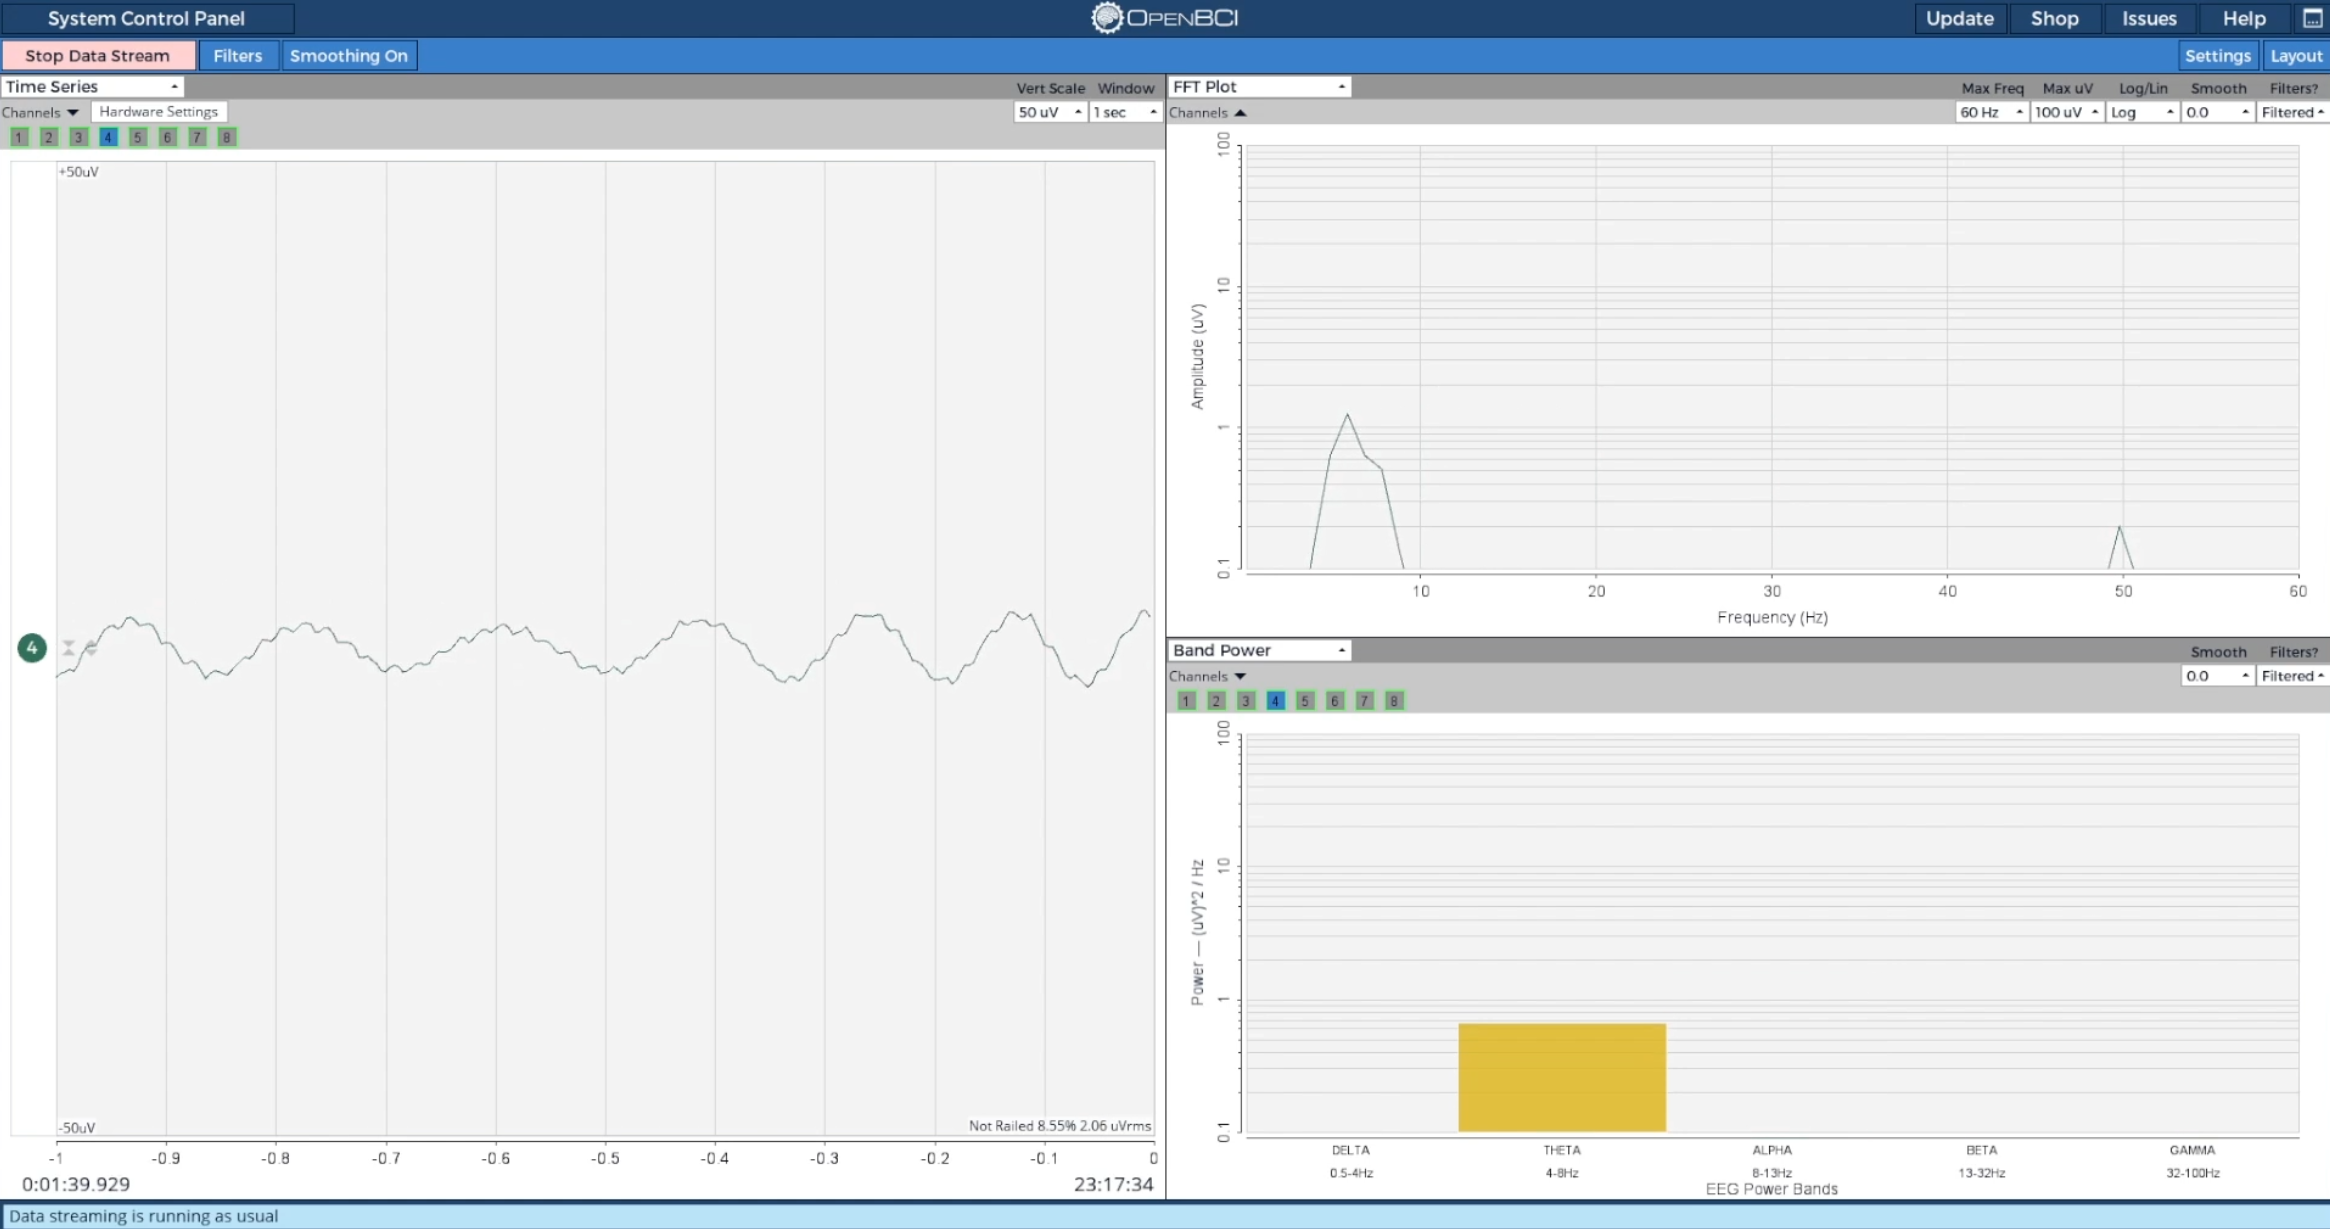
\includegraphics[width=\textwidth]{../../02_Images/freq5.png}
        \caption{5 Hz}
        \label{fig:transduction_5Hz}
    \end{subfigure}
    
    \vspace{0.5cm}
    
    \begin{subfigure}[t]{0.75\textwidth}
        \centering
        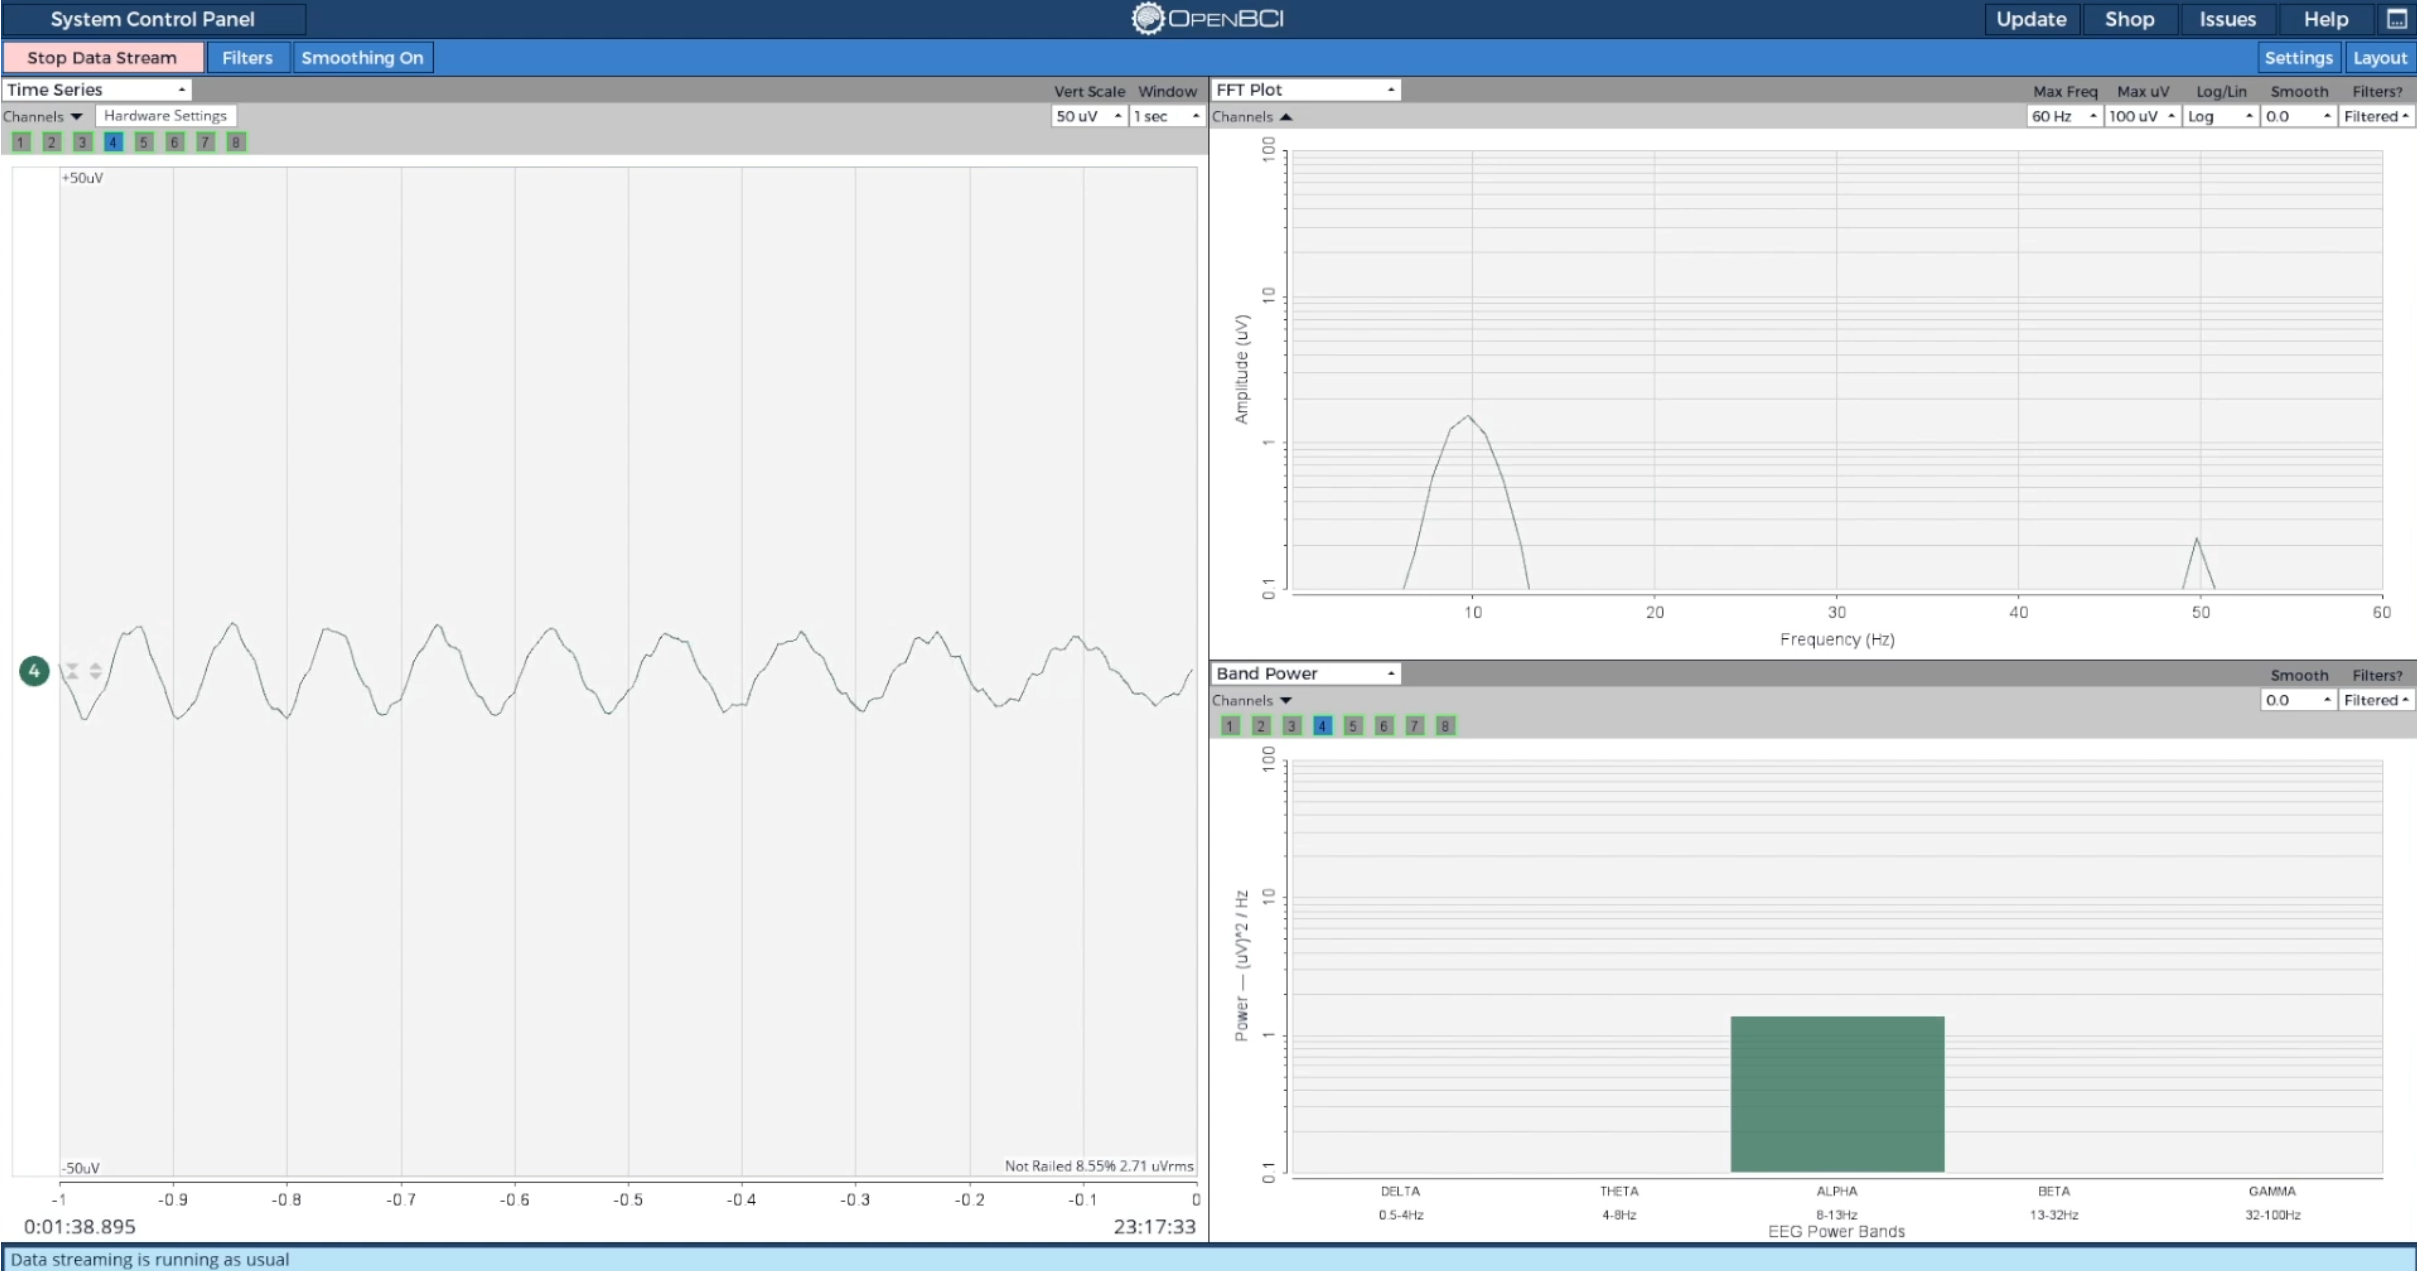
\includegraphics[width=\textwidth]{../../02_Images/freq10.png}
        \caption{10 Hz}
        \label{fig:transduction_10Hz}
    \end{subfigure}
    
    \vspace{0.5cm}
    
    \begin{subfigure}[t]{0.75\textwidth}
        \centering
        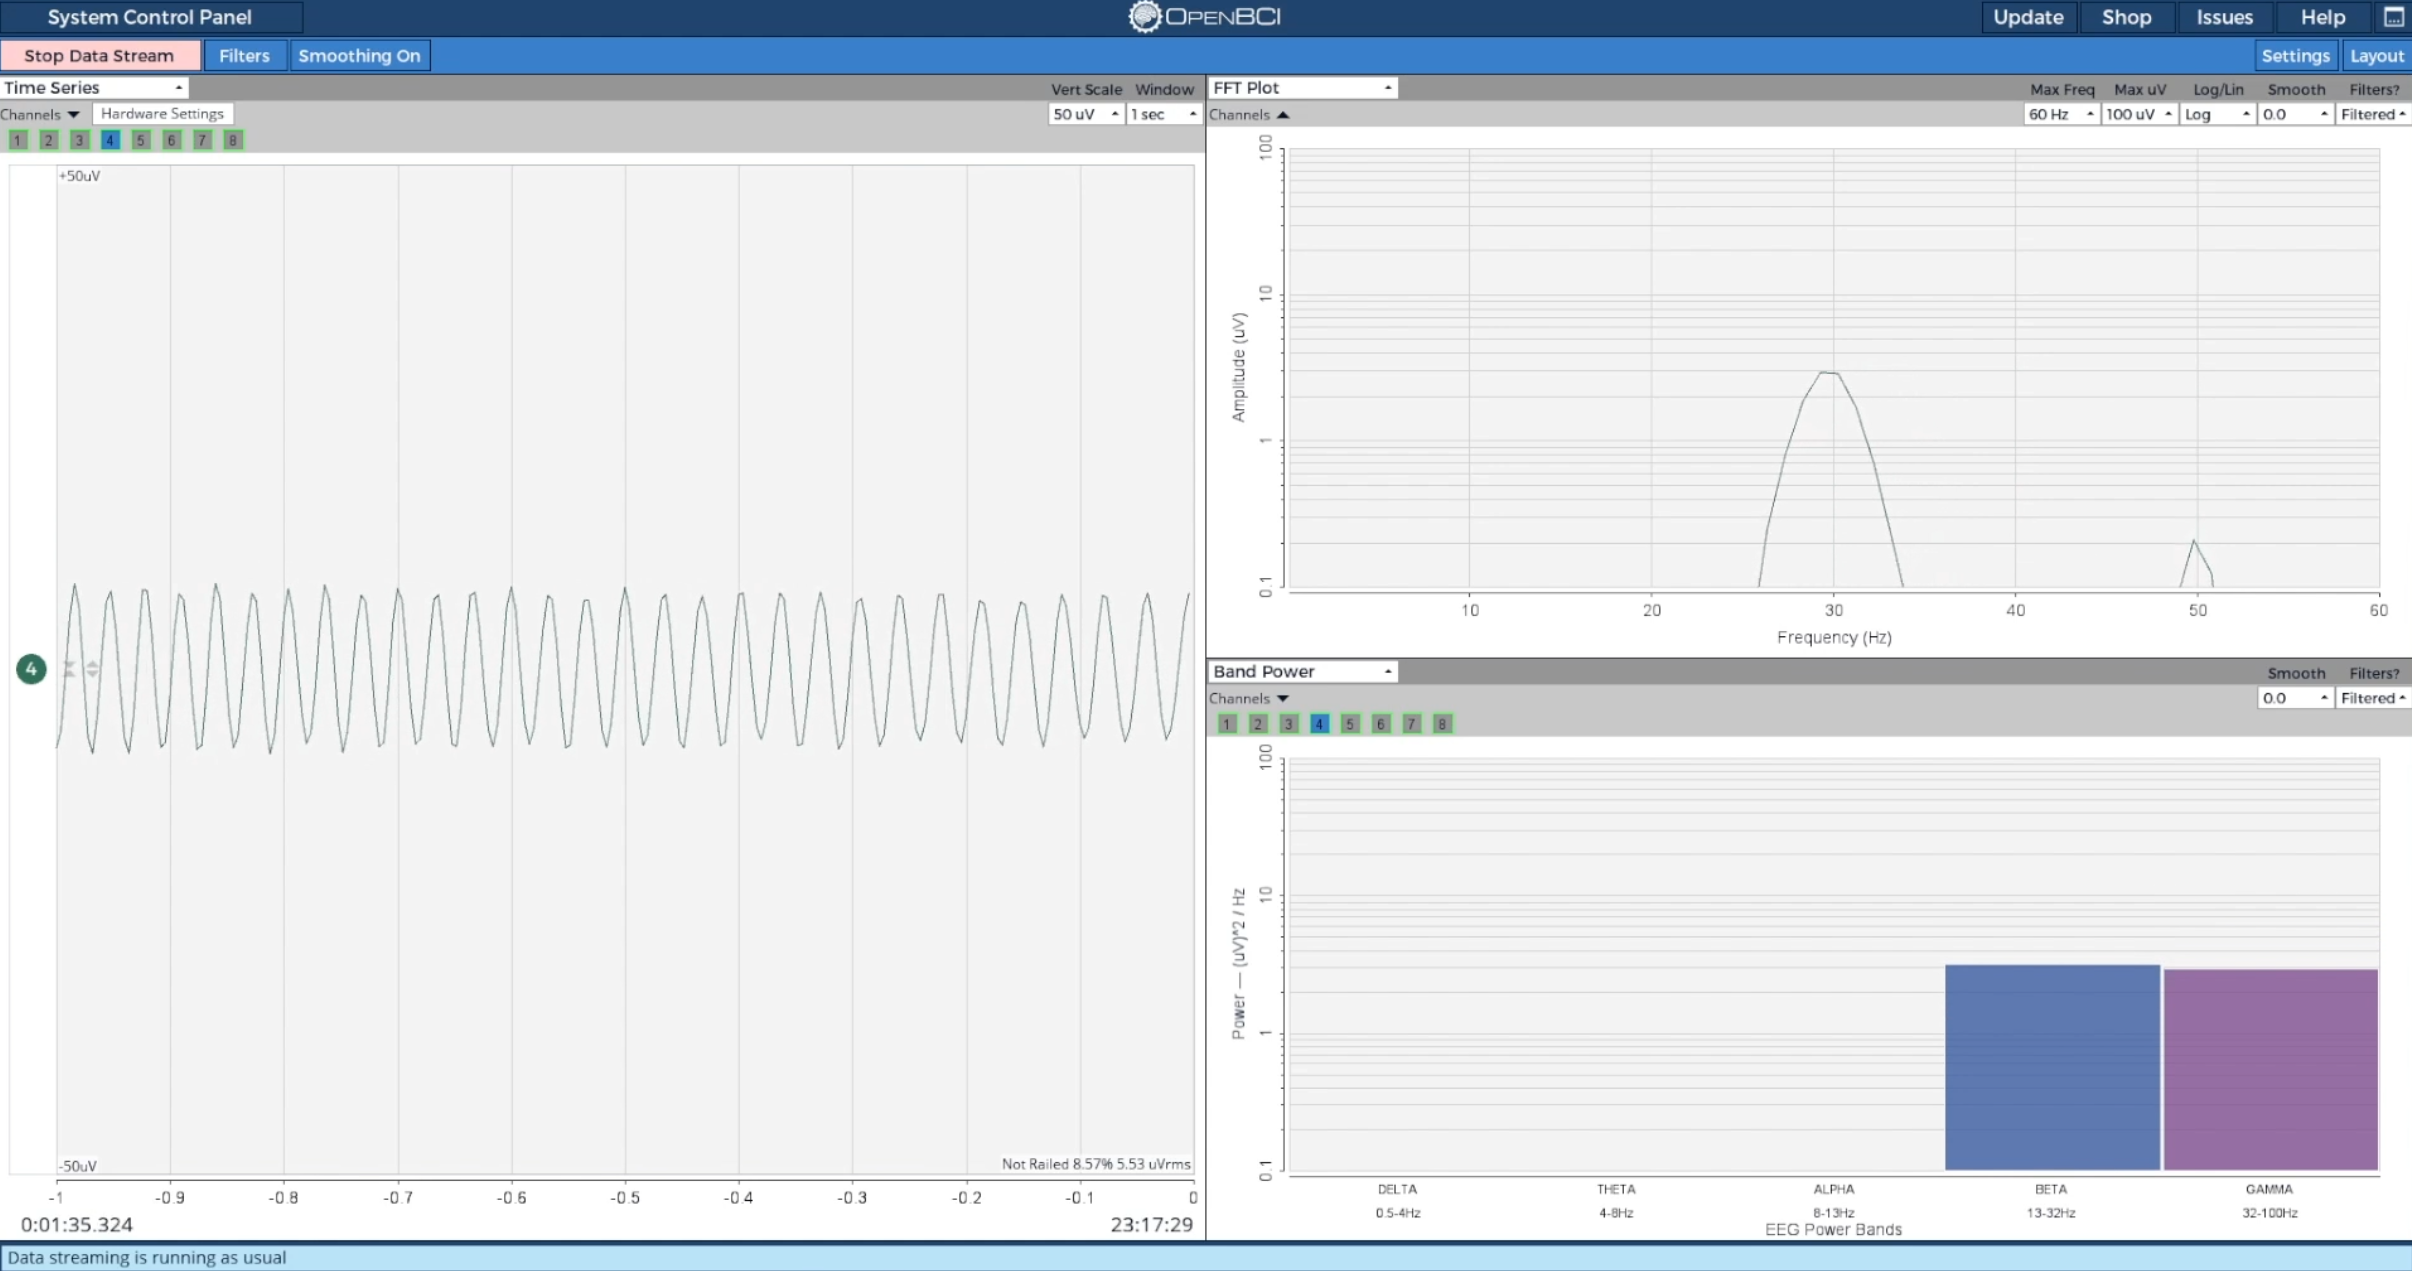
\includegraphics[width=\textwidth]{../../02_Images/freq30.png}
        \caption{30 Hz}
        \label{fig:transduction_30Hz}
    \end{subfigure}
    \caption[Signal Transduction and Attenuation Analysis]{Signal transduction and attenuation analysis results for a gelatine sample with 5\% NaCl concentration at different frequencies.}
    \label{fig:signal_transduction_results}
\end{figure}

\begin{figure}[H]
    \ContinuedFloat
    \centering
    \begin{subfigure}[t]{0.75\textwidth}
        \centering
        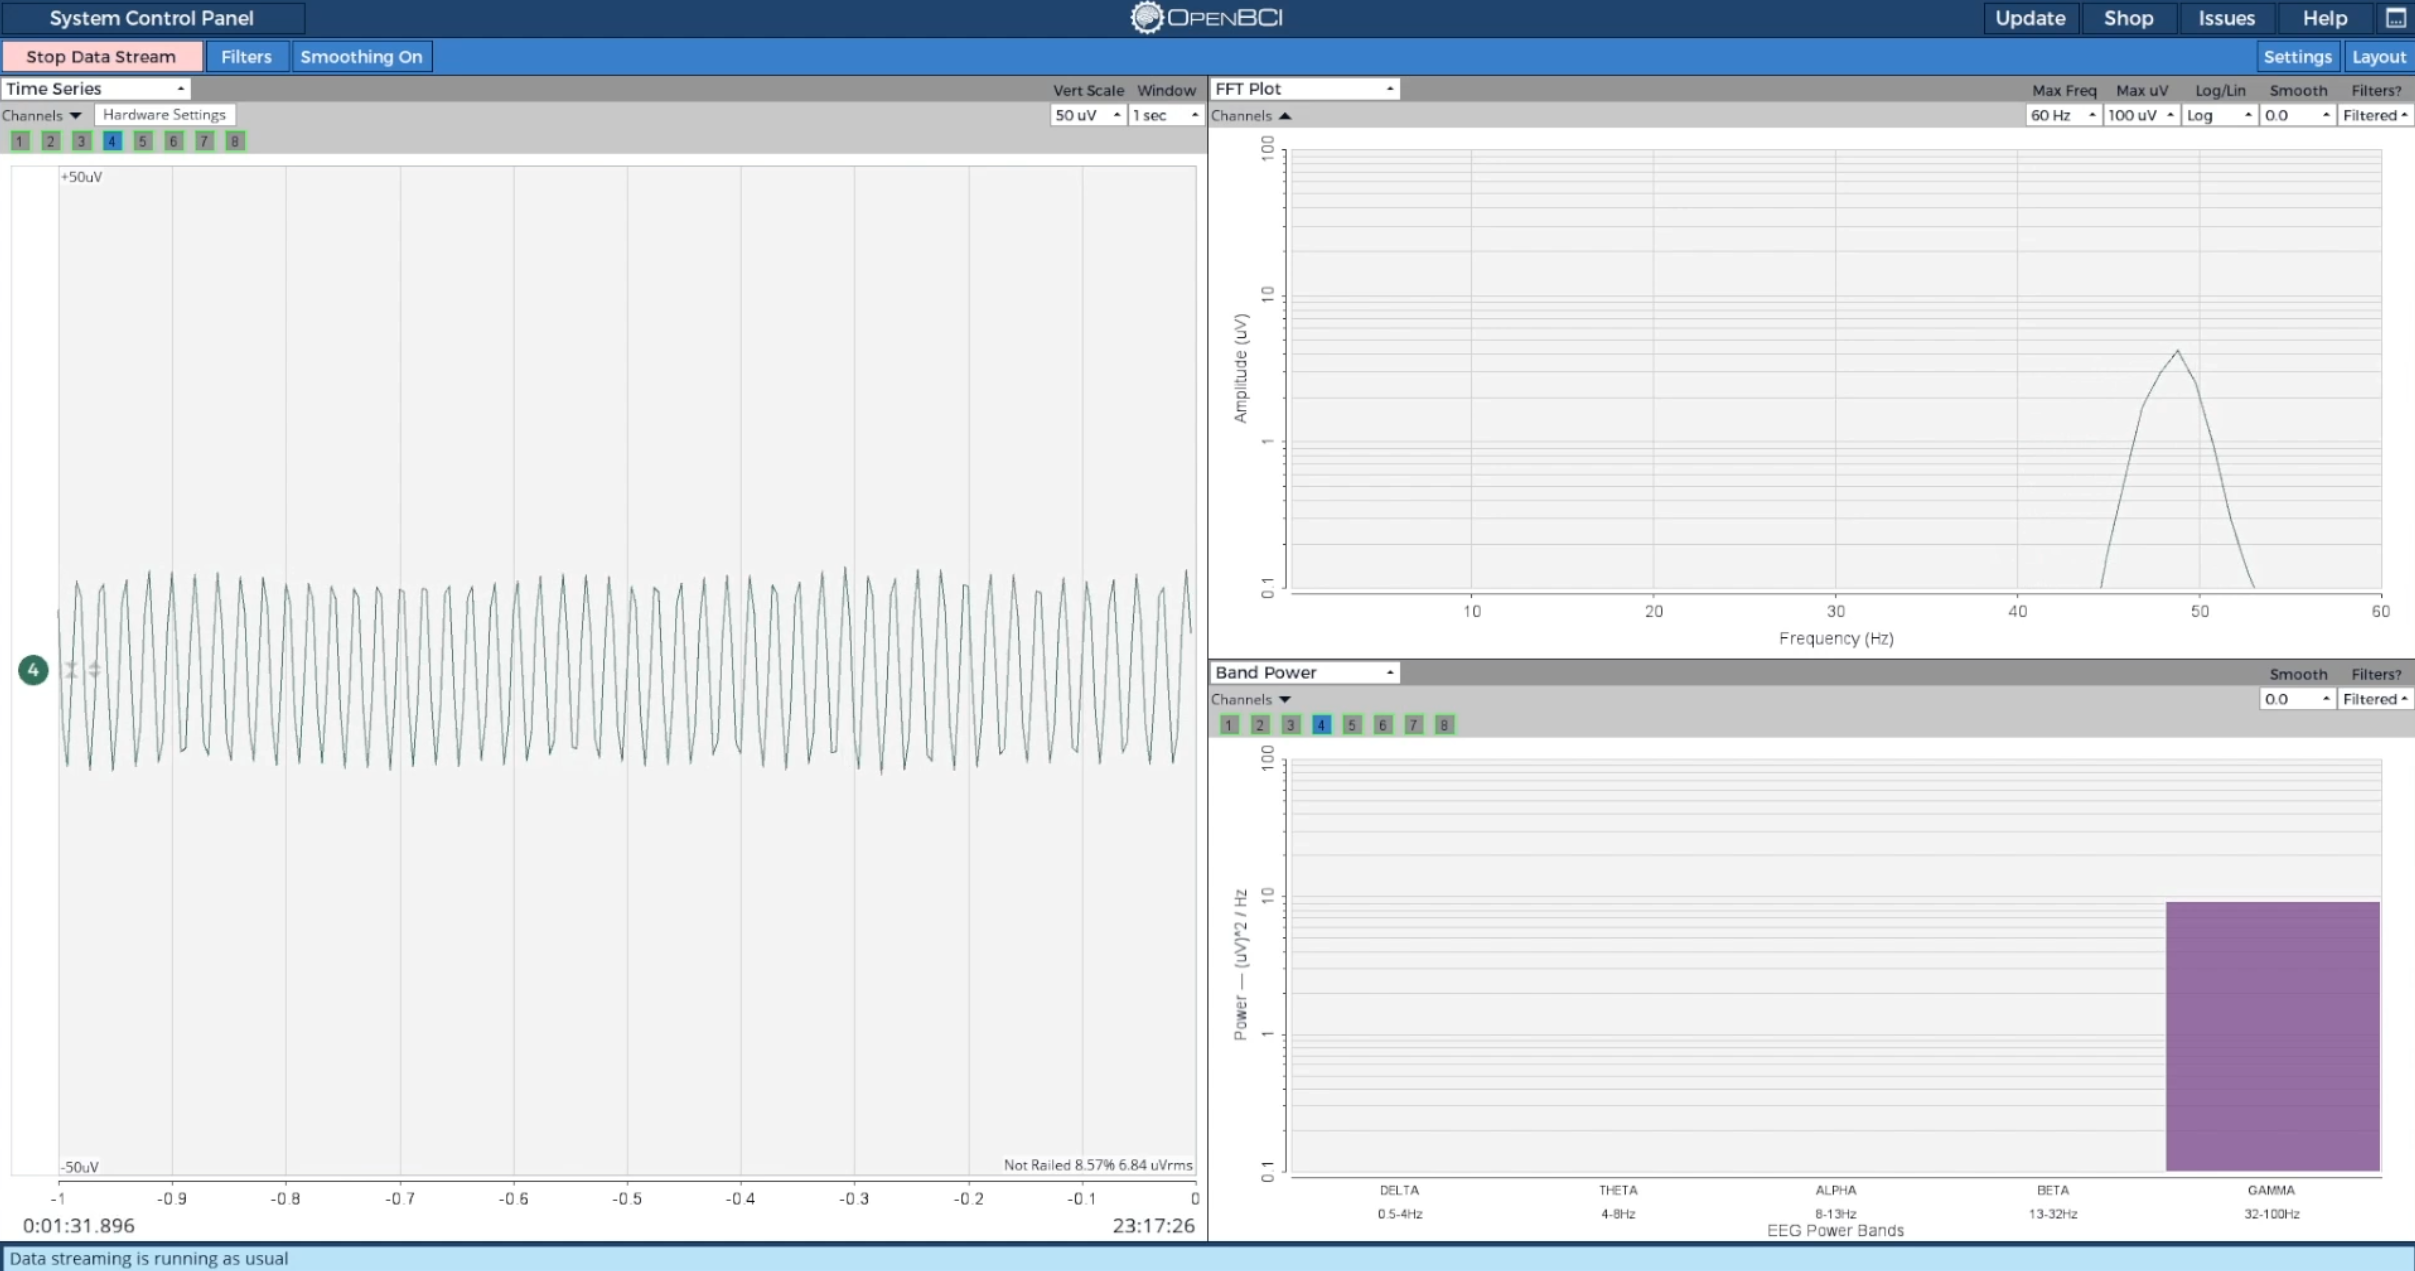
\includegraphics[width=\textwidth]{../../02_Images/freq50.png}
        \caption{50 Hz}
        \label{fig:transduction_50Hz}
    \end{subfigure}
    \caption[]{Signal transduction and attenuation analysis results (cont.).}
\end{figure}
